\subsection{Варианты использования}
	\subsubsection{Регистрация пользователя}
	\begin{enumerate}
		\item Пользователь нажимает кнопку регистрации <<Register>>;
		\item Пользователь вводит логин в поле <<Username>>;
		\item Пользователь вводит пароль в поле <<Password>>;
		\item Пользователь повторяет ввод пароля в поле <<Confirm password>>;
		\item Пользователь нажимает кнопку подтверждения <<Submit>>;
		\item Система регистрирует нового пользователя.
	\end{enumerate}
	
	\textbf{\textit{Альтернатива: этап 5а}} Пользователя с данным логином уже существует: система выдаёт сообщение об ошибке и предлагает выбрать другой логин;
	
	\textbf{\textit{Альтернатива: этап 5б}} Пароли в двух полях не совпадают: Система выводит сообщение об ошибке и просит ввести одинаковые пароли в оба поля.

	\subsubsection{Авторизация пользователя}
	\begin{enumerate}
		\item Пользователь вводит логин в поле <<Username>>;
		\item Пользователь вводит пароль в поле <<Password>>;
		\item Пользователь нажимает кнопку авторизации <<Login>>;
		\item Система уведомляет об успешной авторизации.
	\end{enumerate}
	
	\textbf{\textit{Альтернатива: этап 4}} Пользователя с данным логином и паролем не существует: система выдает сообщение об ошибке и предлагает повторить ввод.
		
	\subsubsection{Получение последней версии документа}
	\begin{enumerate}
		\item Пользователь авторизуется;
		\item Система отображает последнюю версию документа в текстовом поле. Отображаются кнопки управления документом.
	\end{enumerate}
	
	\textbf{\textit{Альтернатива: этап 1}} Пользователя с данным логином и паролем не существует: система выдает сообщение об ошибке и предлагает повторить ввод.
	
	\subsubsection{Получение эксклюзивного доступа}
	\begin{enumerate}
		\item Пользователь авторизуется;
		\item Система отображает последнюю версию документа в текстовом поле. Отображаются кнопки управления документом;
		\item Пользователь нажимает кнопку блокировки <<Lock>>;
		\item Система предоставляет эксклюзивный доступ на редактирование документа.
	\end{enumerate}
	
	\textbf{\textit{Альтернатива: этап 1}} Пользователя с данным логином и паролем не существует: система выдает сообщение об ошибке и предлагает повторить ввод.
	
	\textbf{\textit{Альтернатива: этап 4}} Документ уже заблокирован другим пользователем: Система выдает сообщение об ошибке, эксклюзивный доступ на редактирование не предоставляется.
	
	\subsubsection{Снятие блокировки}
	\begin{enumerate}
		\item Пользователь авторизуется;
		\item Система отображает последнюю версию документа в текстовом поле. Отображаются кнопки управления документом;
		\item Пользователь нажимает кнопку снятия блокировки <<Unlock>>;
		\item Система снимает эксклюзивный доступ на редактирование документа.
	\end{enumerate}
	
	\textbf{\textit{Альтернатива: этап 1}} Пользователя с данным логином и паролем не существует: система выдает сообщение об ошибке и предлагает повторить ввод.
	
	\textbf{\textit{Альтернатива: этап 4}} Документ заблокирован другим пользователем: Система выдает сообщение об ошибке, эксклюзивный доступ остается у предыдущего владельца.
	
 	\subsubsection{Сохранение документа}
 	\begin{enumerate}
 		\item Пользователь авторизуется;
 		\item Система отображает последнюю версию документа в текстовом поле. Отображаются кнопки управления документом;
 		\item Пользователь получает эксклюзивный доступ на редактирования документа;
 		\item Пользователь вносит изменения в текстовое поле документа;
 		\item Пользователь нажимает кнопку сохранения <<Save>>;
 		\item Система сохраняет последнюю версию документа из текстового поля.
 	\end{enumerate}
 	
 	\textbf{\textit{Альтернатива: этап 1}} Пользователя с данным логином и паролем не существует: система выдает сообщение об ошибке и предлагает повторить ввод. Текстовое поле с документом остается пустым;
 	
 	\textbf{\textit{Альтернатива: этап 3}} Документ заблокирован другим пользователем: Система выдает сообщение об ошибке, эксклюзивный доступ остается у предыдущего владельца, содержимое документа не изменяется;
 	
 	\textbf{\textit{Альтернатива: этап 6}} Пользователь не обладает эксклюзивным доступом: Система выдает сообщение об ошибке и просит получить эксклюзивный доступ перед сохранением документа.
	
\subsection{Модель предметной области}
	\begin{figure}[H]
		\centering
		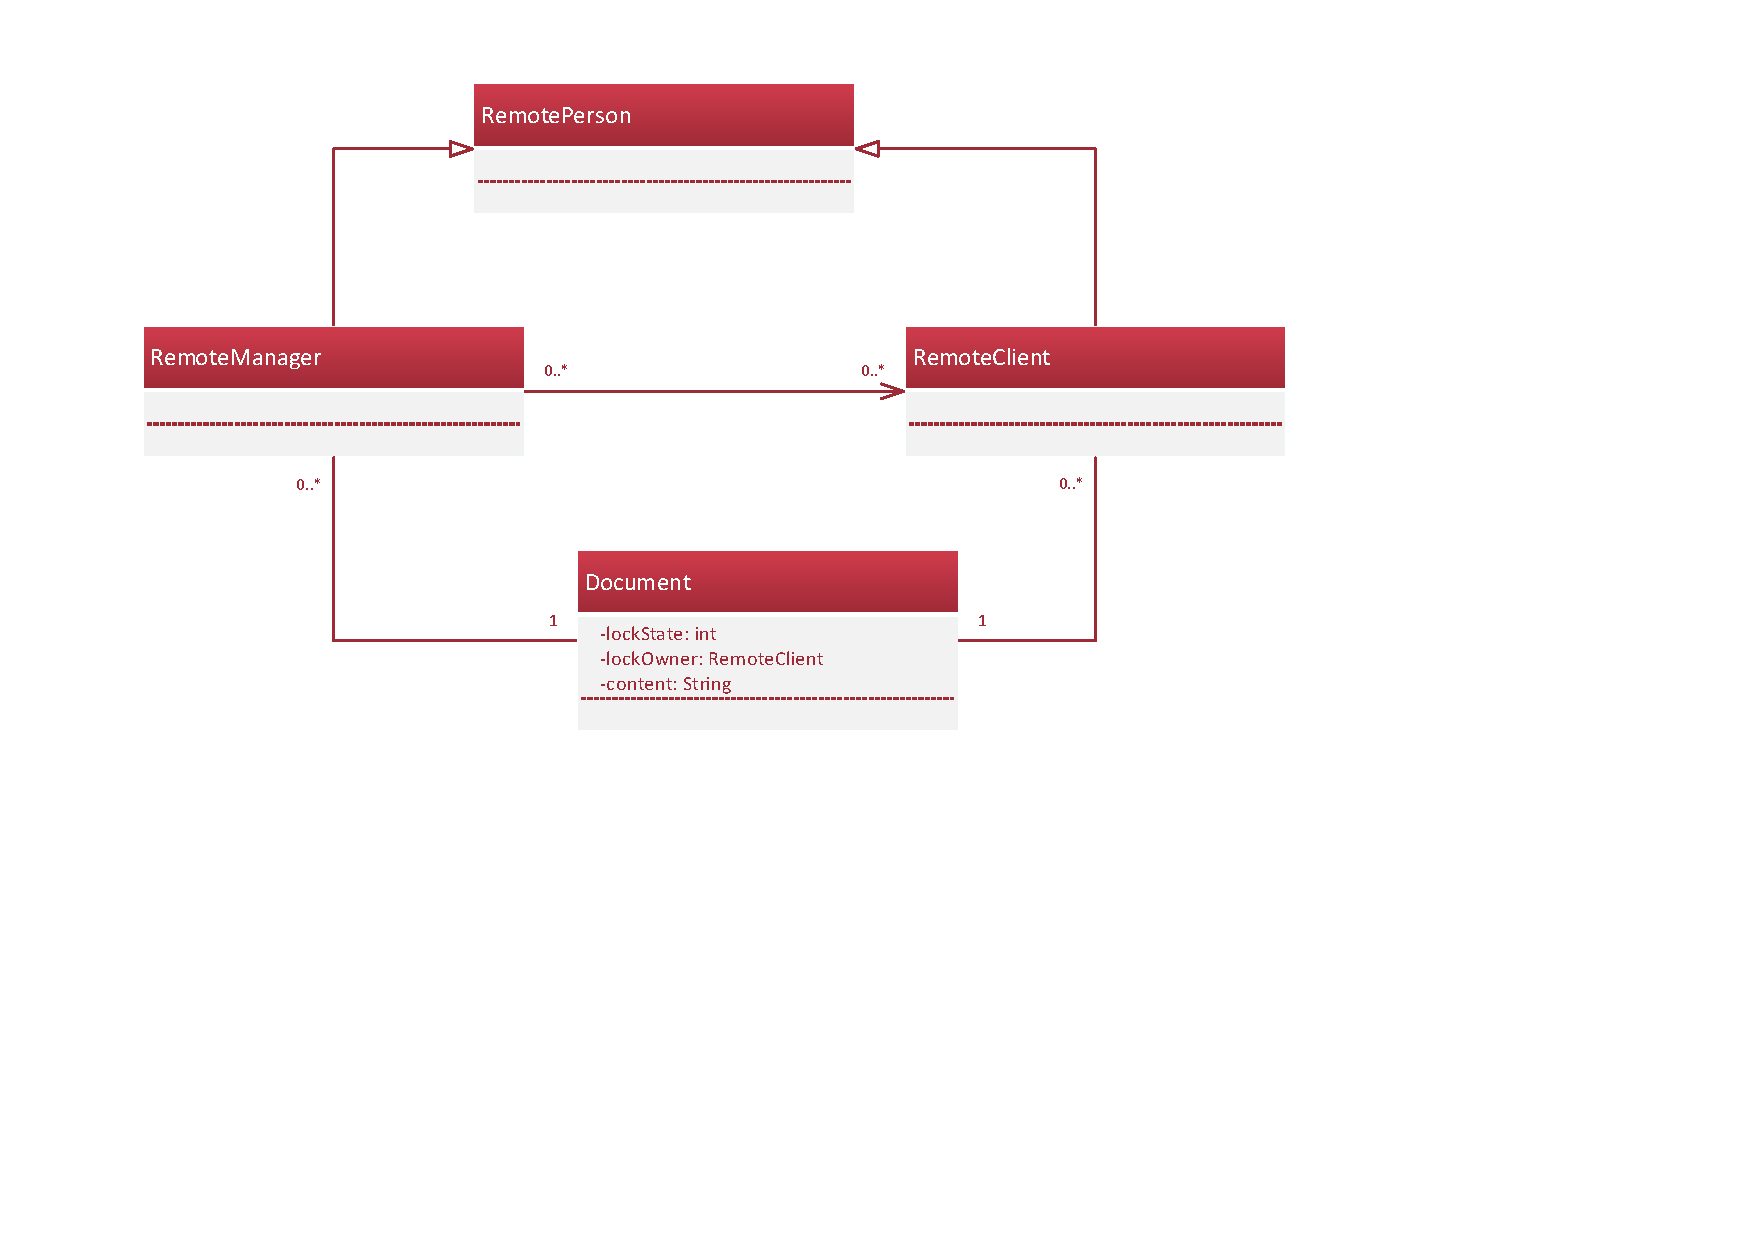
\includegraphics[width=1\textwidth]{EPDiagram}
		\caption{Модель предметной области}
		\label{fig:class_ob}
	\end{figure}